\section{Nuværende omkostninger i sundhedssektoren}
Det er relevant at se på omkostningerne i både den primære og sekundære sundhedssektor i forhold de nuværende målemetoder der bliver anvendt til fysisk aktivitet hos patienter med hypertension, for at give et indtryk af hvilke områder der vil kunne berøres, hvis en implementering af Fitbit Flex bliver en realitet. 

\subsection{Primær sektor} \label{sec:nuv_primaer}
\label{sec:primaer_sektor_omkostninger}
Den subjektive målemetode, der på nuværende tidspunkt benyttes af $27,7~\%$ af praktiserende læger, foregår ved spørgeskema under en konsultation, medfører udgifter i den primære sundhedssektor \citep{munck2007}. Afhængigt af antal konsultationer, som den enkelte kroniker har behov for, kan omkostningerne i forbindelse med konsultation ved udfyldelse af spørgeskemaer stige, mens udarbejdelse og udskrifter af spørgeskemaer vil have relativt lave omkostninger.
\citeauthor{munck2007} udarbejdede i 2007 en rapport om hypertension i almen praksis. Her blev $159$ kontaktpersoner i almen praksis spurgt: \textit{"Sætter I jeres hypertensionspatienter til kontrol med fast tidsinterval? Hvis ja, angiv det typiske interval"}. Her svarede $92,5~\%$, at de sætter deres patienter til kontrol med et fast tidsinterval, hvor den gennemsnitlige interval er udregnet til $3,9$ måneder \citep{munck2007}. 

Hvis det, jævnfør \citeauthor{kronborg2008}, antages at $1/5$ af den voksne danske befolkning har hypertension, vil dette svare til omkring $900.000$ danskere \citep{folketal2016}. Hvis $900.000$ danskere skal til lægekonsultation á $137,93$ kroner hver $3,9$. måned, vil dette svare til en årsomkostning for sundhedssektoren på omkring $380$ millioner kroner \citep{honorartabel2016}. 

Den samlede medicinudgift i den primære sundhedssektor i Danmark i $2014$ lå på $11,6$ milliarder kroner, og Danmarks Statistik påpeger i denne sammenhæng, at blodtrykssænkende medicin og hjertemedicin er nogle af de mest anvendte former for medicin i Danmark \citep{dst2016}. Yderligere har de danske regioner udgifter til medicintilskud, der ydes til patienter med høje omkostninger til medicin. I $2014$ havde regionerne $5.606$ millioner kroner i udgifter til medicintilskud, hvilket var en stigning i forhold til det foregående år \citep{medicinoekonomi2015}. Dette skyldes blandt andet ny, dyr, medicin, samt at flere patienter med kroniske lidelser behandles med medicin, hvorfor mængden af medicin stiger, og skaber flere udgifter for regionerne \citep{regioner2015}. 

Ifølge en rapport udarbejdet af \citeauthor{apotekerforeningen2012} oplyses de mest udleverede blodtrykssænkende lægemidler i 2012 opgjort i Definerede DøgnDoser (DDD). Her fremgår, at Amlodipin (139 millioner DDD), Furosemid (94 millioner DDD), Ramipril (92 millioner DDD), Bendroflumenthiazid og kalium (85 millioner DDD), Enalapril (80 millioner DDD), samt Losartan (73 millioner DDD) er de blodtrykssænkende lægemidler med flest udleverede døgndoser. Dette svarer til samlet $563$ millioner DDD i $2012$ for disse blodtrykssænkende lægemidler \citep{apotekerforeningen2012}. DDD beskriver den gennemsnitlige anbefalede døgndosis, hvilket bruges til at sammenligne priser på forskellige lægemidler, og i $2012$ blev i alt udstedt $2.343$ millioner DDD \citep{medicinoekonomi2015}. 

Hvis aktivitetsarmbånd som en non-farmakologisk  behandling implementeres i den almene praksis, vil antallet af DDD kunne mindskes for patienter med hypertension, såfremt implementeringen påvirker patienternes helbred og blodtryk positivt. Ud over besparelser på DDD vil bivirkninger ved lægemidlerne også kunne reduceres, hvilket vil resultere i bedre livskvalitet for patienterne, samt et lettere behandlingsforløb. Eksempler på de hyppigste bivirkninger ved de fleste af de nævnte lægemidler er ødemer, dehydrering, træthed, hovedpine og svimmelhed \citep{olsen2015}. Den bedste medicinering mod hypertension er individuel, hvorfor det ofte er nødvendigt at finde de lægepræparater, der er mest effektive for den enkelte patient, uden at der er for mange bivirkninger, hvilket besværligør og forlænger patienternes behandling.

\subsection{Sekundær sektor}
Den sekundære sektor påvirkes også af hypertension, da sygdommen er skyld i ambulante besøg og indlæggelser. I $2014$ var der $49.875$ ambulante besøg i den offentlige sekundære sektor for patienter med diagnosen blodtryksforhøjelse af enten kendt eller ukendt årsag, hvilket svarer til en stigning på $8,35~\%$ siden $2012$, hvilket kan ses på \autoref{fig:hyp_sekundaer} \citep{sundhedsdatastyrelsen2016}. 

\begin{figure}[H]
\centering
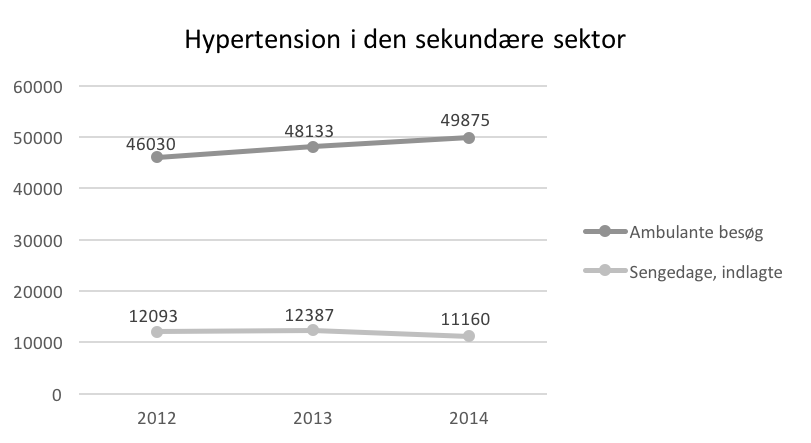
\includegraphics[width=0.8\textwidth]{figures/hyp_sekundaer}
\caption{Henvendelser i den offentlige sekundære sektor som følge af hypertension fra 2012 til 2014 \citep{sundhedsdatastyrelsen2016}.}
\label{fig:hyp_sekundaer}
\end{figure}

\noindent
Yderligere havde patienter med hypertension $11.160$ sengedage i forbindelse med indlæggelse på offentlige sygehuse i $2014$, hvilket var et fald i forholdt til de to foregående år \citep{sundhedsdatastyrelsen2016}. 

Jævnfør \citeauthor{takstvejledning2016} er taksten for et ambulant besøg  med journaloptagelse $1.421$ kroner uden nogen særlige procedurer, og taksten for en indlæggelse af en patient med hypertension er $12.597$ kroner indtil fire dage, der er det maksimale antal sengedage, der er dækket af denne takst. Ud over fire dage kan der opkræves en brugerbetaling for langliggertakst på $1.976$ kroner \citep{takstvejledning2016}. 

Hvis det antages, at ambulante besøg og antal sengedage i $2014$ er tilsvarende til henvendelser i år $2016$, så vil prisen for dette være omkring $210$ millioner kroner for ét år. 